\section{Digitalisierung}
Ablauf einer PCM (Pulse-Code-Modulation) sind Sampling, Quantisierung mit anschliessender Codierung. Digitalisierung sind diese drei genannten Schritte.

Vorteile gegenüber Analogen Signalen sind bessere Signalübertragung, einheitliche Speicherung, Reproduzierbare Probleme und auch zB möglicher Datenschutz.

\subsection{Sampling}
\subsection{Natural Sampling}
\textbf{Zeitbereich} \script{73}:\\
In jedem Intervall $T_s$ wird $m(t)$ auf den Abtastwert $m_{NS}(k\cdot T_s)$ reduziert. Die reelle mathematische Funktion lautet:
\begin{align*}
	\text{rect}_{T_s}\left(\frac{t}{\tau}\right) &= \sum_{n=-\infty}^{\infty}\text{rect}\left(\frac{t - n\cdot T_s}{\tau}\right) \\
	m_{NS}(t) &= \frac{1}{\tau}m(t)\cdot\text{rect}\left(\frac{t}{\tau}\right)
\end{align*}

Für eine ideale Abtastung im Zeitbereiche kann folgende Funktion verwendet werden:
\[
m_s(t) = m(t)\cdot \delta_{T_s}(t)
\]

\textbf{Beispiel} mit $\tau = \frac{T_s}{2}$\\
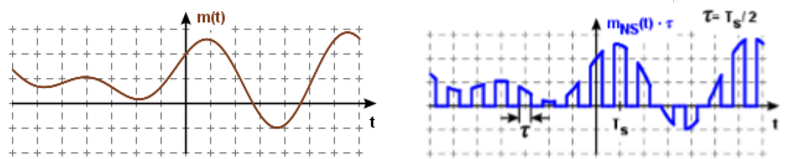
\includegraphics[width=\columnwidth]{Images/natural_time}
~\\
\textbf{Frequenzbereich} \script{74}:\\
Solang die Pulsbreite $\tau$ nicht unendlich Kurz ist (kein Dirac-Stoss), werden die Frequenz gegen 0 streben. Die wiederholten Spektren dürfen sich \underline{nicht} überlagern, ansonsten entstehen Alaising-Effekte welche nur durch ein höhere Abtastung behoben werden kann. Dies bedeutet für die reale mathematische Funktion:
\[
M_{NS}(\omega) = \frac{1}{T_s}\sum_{n=-\infty}^{\infty}\frac{\sin\left(\frac{n\pi\tau}{T_s}\right)}{\frac{n\pi\tau}{T_s}}\cdot M(\omega - n \omega_s)
\]

Für die ideale Abtastung im Frequenzbereich:
\[
M_s(\omega) = \frac{1}{T_s}\sum_{n=-\infty}^{\infty}M(\omega -n\omega_s)
\]

\textbf{Beispiel} mit $\tau = \frac{T_s}{2}$\\
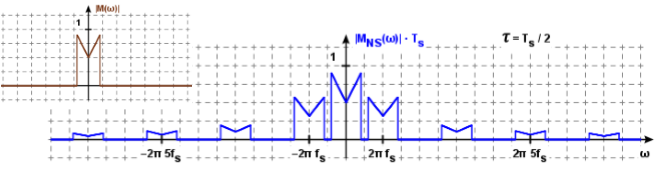
\includegraphics[width=\columnwidth]{Images/natural_freq}

\subsection{Nyquist-Shannon Abtasttheorem}
Die minimale Samplerate $f_s$ für \textbf{alaising}-freie Abtastung $f_{S_N}$ eines Basisbandsignals \script{76}:
\[
f_s > f_{S_N} = 2 \cdot B_m
\]

Die \textbf{Nyquist-Frequenz} $f_N = \frac{1}{2}f_s$ ist die maximale Frequenz welche im Signal vorkommen kann und das \textbf{Nyqust-Intervall} $T_{S_N} = T_S < T_{S_N} = \frac{1}{f_{S_N}} = \frac{1}{2B_m}$ die maximale Intervallgrösse für alaising-freie Basisband-Abtastung. Diese können auch in Nyquest-Zonen eingeteilt werden.

\subsection{Rekonstruktion}
Das Ursprüngliche Nachrichtensignal $m(t)$ kann im Frequenzbereich mit der Summe der gewichtetet Abtastwerten einzelner $h_{LPF}$ Funktionen berechnet werden. 
\[
h_{LPF}(t) = T_s \cdot \frac{\omega_s}{2\pi}\cdot\frac{\sin(2\pi\cdot f_c \cdot t)}{2\pi\cdot f_c \cdot t}
\]
Exakte Rekonstruktion von $m(t)$ durch LPF mit Eckfrequenz $f_c$:
\[
m(t) = \sum_{m=-\infty}^{\infty}m_s(k\cdot T)\frac{\sin(2\pi \cdot f_s \cdot (t -k\cdot T_s))}{2\pi \cdot f_s \cdot (t -k\cdot T_s}
\]
D/A Wandler verwenden dazu den \textbf{Zero-Order Hold} im Frequenzbereich mit Pulsbreite $\tau = T_s$:
\[
H_{ZOH}(\omega) = \tau \cdot \frac{\sin(\frac{\omega\tau}{2})}{\frac{\omega\tau}{2}}
\]

\noindent Die \textbf{Dämpfung} $d$ einer Zero-Order Hold $H_{ZOH}(\omega)$ ergibt sich mit $d = 20\cdot \lim\limits_{min \rightarrow 0} \left(\log_{10}\left|\frac{H_{ZOH}(max)}{H_{ZOH}(min)}\right|\right)$

\subsection{Quantisierung}\script{80}
Anzahl Bit pro Codewort eines digitalen Signals muss endlich sein und wird bei \underline{gleichförmiger Quantisierung} in gleichen Schritten verteilt. Die Auflösung (Anzahl bit) $n$ und Quantisierungsstuffe $L =2^n$ bzw. \textbf{Quantisierungsintervall} $\Delta = \frac{max - min}{L}$. Der \textbf{Quantisierungsfehler} $q_{e} = \frac{\Delta}{2}$

~\\
\noindent\textbf{Beispiel:} CD
$n = 16$ bit/sample, $L=2^{16} = 65536$ und $\Delta = 30.5\mu V$

Der Quantisierungsfehler $q_e$ besitzt eine mittlere Leistung $\overline{P}_q = \frac{\Delta^2}{12}$. Das Leistungsverhältnis von Nutz- zu Störsignal \textbf{SNR} kann berechnet werden, wobei $C$ der Scheitelfaktor ist:
\[
SNR_q = \frac{S}{N_q} = \frac{m_{rms}^2}{\overline{P}_q} = \frac{3}{C^2}\cdot2^{2n}
\]
$SNR_q$ in dB mit Anzahl bits $n$:
\[
SNR_q = n\cdot 6.02 + 10\log_{10}\left(\frac{3}{C^2}\right)dB
\]

Dabei ist zB auf einer CD der Scheitelfaktor $C = \sqrt{2}$, weil dies mit einem Sinussignal verglichen werden kann. 
